\subsection{(Pending funding) Designing addressable self-assembly for bio-inspired information storage}

%\begin{figure}[t!]
%\begin{center}
%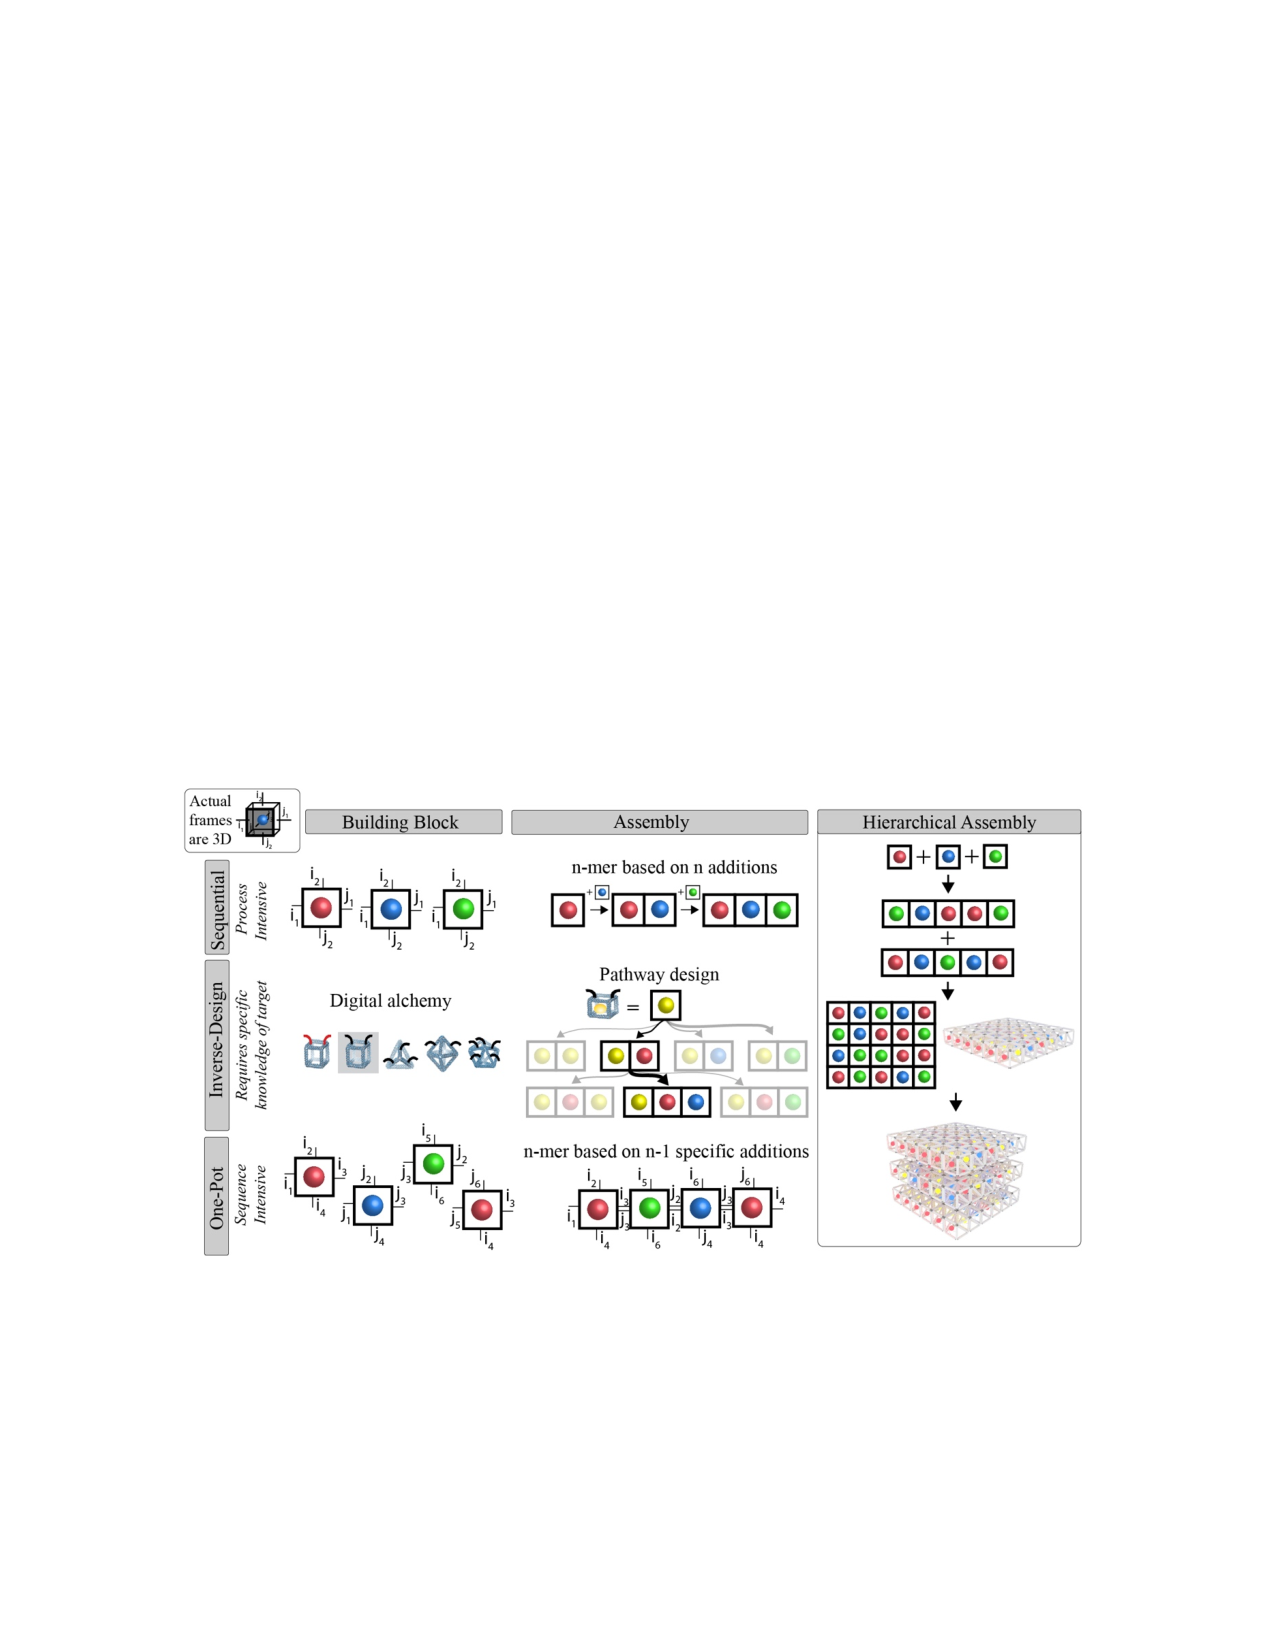
\includegraphics[width=6.5in]{../figures/SemiSynBio.pdf}
%\caption{
%Strategies for building information encoded 1D, 2D and 3D arrays. Sequential operations are very deterministic and can be carried out by automated robotic equipment, but even so are heavily process intensive and require many individual assembly steps. One-pot systems can be fully computationally defined, though in practice are heavily sequence intensive and be subjected to errors more readily than in molecular-scale systems when accounting for kinetic and thermodynamics of packing larger objects and materials. A hierarchical assembly methodology offers a hybrid approach of both strategies, where a sequential addition of structures preformed in a one-pot setup provide the desired 3D material organization.}
%\label{fig:semisynbio}
%\end{center}
%\end{figure}

\textit{Background}

The following work draws from a National Science Foundation (NSF) proposal for Semiconductor Synthetic Biology for Information Processing and Storage Technologies (SemiSynBio), submitted October 2017 and pending funding.
If funded, this collaboration would include the groups of Mark Bathe (MIT), Moungi Bawendi (MIT), and Oleg Gang (Columbia).

We proposed using DNA Memory Blocks (DNAMB) as our monomer units of information, which we could then addressably assemble into arrays for storage. 
Within each DNAMB monomer, multiple units of memory can be contained: blocks are composed of a DNA cage which can encapsulate a variety of memory blocks (e.g. Au NP, QDs, fluorescent dyes).
To self-assemble these systems into 2D and 3D ultra-dense data blocks, we will investigate the minimum interaction specificity needed to direct self-assembly into high fidelity ordered 2D and 3D arrays.

1. Digital alchemy for shape
2. Want to design sufficiently specific interaction
In this way, we can inversely design ideal DNA cages (e.g. shape, patchy interactions) that will robustly assemble a target structure. We will seek to balance site specificity without being overly unique?that is, design the highest information interactions that will allow for the minimum amount of linkage specificity for directing self-assembly84,85.

Sub-Aim 2.2. Hierarchical assembly logic for higher-dimensional information storage
We will explore several complementary approaches to hierarchical assembly engineering, including sequential nanoparticle addition and ?one-pot assembly?, each of which will be explored together with inverse computational design of self-assembly pathways and particle geometries to achieve a robust assembly of designed arrays. 

Assembly of encoded 3D arrays can be approached in two strategies, or a combination thereof. In an entirely ?one-pot? assembly of a 3D array, all modules are linked with a large binding sequence set that has been fully computationally defined. Such an approach requires an enormous number of unique binding sequences, and even if fully defined, can run into high error rates when considering the assembly and packing of large (as compared with molecular assembly) and charged modules and/or materials. A second approach using sequential binding based on module groups of similar binding layouts requires less sequence diversity and can be automated using robotic liquid handling. However, this is vastly more process- and time-intensive than one-pot assembly. This approach represents hierarchical assembly, whereby 1D structures (?strings?) would be formed from the modules, 2D planes formed from the 1D libraries, and finally 3D encoded arrays from stacking of selected planes. An optimal assembly process that balances fully-encoded organization with direct addition of binding components would offer a hybrid approach of hierarchical assembly with sequential addition of groupings of computationally defined structures. Each of these strategies will be explored in this aim, using a combination of high-throughput, structure-based computational modeling and experiments.

The Glotzer group will extend their digital alchemy framework to probe diverse DNA linkage sequences and conjugation designs to realize specific, targeted inter-particle interactions. In addition, they will explore the roles of these interactions on the kinetics of array assembly to enable pathway design \cite{Jankowski_2012_SoftMatter} into desired arrays while avoiding undesirable ?side products?. In this way, we will explore computationally the interplay between the two extremes of one-pot and sequential assembly, and identify which combinations provide lowest assembly error while minimizing both assembly time and the number of required unique binding sequences.


%\textit{From intro}:
%In Aim 1, we will investigate monomeric block formation, exploring the self-assembly of arbitrary geometric DNA objects with incorporated optical elements that can be manufactured as information carriers, while allowing for superstructure formation through DNA-sequence barcoding. We will explore static assembly of 1D arrays of such DNA nanoparticles integrated with Memory Blocks (DNAMB) for encoding bitstream information that can be read out by fluorescence and electron microscopy. In Aim 2, we will explore 2D and 3D assembly, investigating techniques to algorithmically assemble and read out digital 2D and 3D information using optical and tomographic methods. In Aim 3, we will use molecular decision computing to assemble distinct, alternative lattices based on specific external signals. These results will offer the ability to encode and decode arbitrary datasets in ultra-dense molecular hard-drives, with environmental sensing and recording.

%Aim 2. Dense, programmable molecular memory in 2D and 3D bit module lattice assemblies
%Overview \& Rationale. Nanoparticle self-assembly depends on a balance of interaction forces, entropic effects, and system kinetics37,53,69-73. We can leverage these properties to direct self-assembly of shaped DNA nanoparticle into 2D and 3D arrays by controlling the position and valency overhangs that provide connectivity between DNA nanoparticles. Wireframe structure of DNA particle is highly suitable for encapsulation of memory blocks (e.g. Au NP, QDs, fluorescent dyes) and creation of DNAMB, a pixel in 2D or 3D arrays. To achieve information storage capabilities, it is required to investigate how the connectivity properties of DNAMB can be translated into their designed arrangement in the information- storing arrays. To self-assemble these systems into 2D and 3D ultra-dense data blocks, we will investigate the minimum interaction specificity needed to direct self-assembly into high fidelity ordered 2D and 3D arrays. We will also explore information retrieval from these arrays in 2D and 3D within pixels consisting of 1x1, 2x2, 4x4, etc., nanoparticle block arrays. In addition, we will establish methods for generating robust memory arrays that can preserve information under extreme conditions.

%\textit{Proposed research, Aim 1}: Computationally, Glotzer and colleagues will develop a bit module interaction model to study the role of the DNA linkages on DNA cage self-assembly. Specifically, previous work on modeling solid particles with DNA-facilitated attraction37 will be extended to model the DNA cages that will be experimentally made by Gang, and it will consider realistic features of nanoparticle systems82,83. With this model in place, we can then extend the framework of digital alchemy, which treats particle properties as a thermodynamic variable, to particle interactions (here, DNA linkages)54. In this way, we can inversely design ideal DNA cages (e.g. shape, patchy interactions) that will robustly assemble a target structure. We will seek to balance site specificity without being overly unique?that is, design the highest information interactions that will allow for the minimum amount of linkage specificity for directing self-assembly84,85. This computational framework for the inverse design of bit packages that will assemble a given structure will enable high- throughput screening of particles of interest and serve as the basis for complex hierarchical structure and array assembly in the remainder of Aims 2 and 3.

%Sub-Aim 2.2. Hierarchical assembly logic for higher-dimensional information storage
%Overview. In Sub-aim 2.1, we explored approaches to assembling DNA frames into target 2D and 3D assemblies. Next, we precisely order ?bit modules??that is, DNA cages carrying functional particles? into arrays of discrete information. Toward this end, we design modules that carry the minimal information needed to reach target arrangements through a combination of particle anisotropy and DNA linkers. DNA computing groups have previously used DNA linkers to self-assemble complex 2D patterns6 and 3D shapes9. Here we extending these approaches to realize hierarchical 3D nanoparticle assembly design so that pixelated images act as dense data storage units. We will explore several complementary approaches to hierarchical assembly engineering, including sequential nanoparticle addition and ?one-pot assembly?, each of which will be explored together with inverse computational design of self-assembly pathways and particle geometries to achieve a robust assembly of designed arrays. Using the optical characterization strategies from Sub-aim 2.1, we will decode the information encoded in the structure, and probe sources of error and information loss in the self-assembly and read-out processes.

%\textit{Proposed research}. Assembly of encoded 3D arrays can be approached in two strategies, or a combination thereof (Fig. \ref{fig:semisynbio}). In an entirely ?one-pot? assembly of a 3D array, all modules are linked with a large binding sequence set that has been fully computationally defined. Such an approach requires an enormous number of unique binding sequences, and even if fully defined, can run into high error rates when considering the assembly and packing of large (as compared with molecular assembly) and charged modules and/or materials. A second approach using sequential binding based on module groups of similar binding layouts requires less sequence diversity and can be automated using robotic liquid handling. However, this is vastly more process- and time-intensive than one-pot assembly. This approach represents hierarchical assembly, whereby 1D structures (?strings?) would be formed from the modules, 2D planes formed from the 1D libraries, and finally 3D encoded arrays from stacking of selected planes. An optimal assembly process that balances fully-encoded organization with direct addition of binding components would offer a hybrid approach of hierarchical assembly with sequential addition of groupings of computationally defined structures. Each of these strategies will be explored in this aim, using a combination of high-throughput, structure-based computational modeling and experiments.

%The Glotzer group will extend their digital alchemy framework to probe diverse DNA linkage sequences and conjugation designs to realize specific, targeted inter-particle interactions. In addition, they will explore the roles of these interactions on the kinetics of array assembly to enable pathway design \cite{Jankowski_2012_SoftMatter} into desired arrays while avoiding undesirable ?side products?. In this way, we will explore computationally the interplay between the two extremes of one-pot and sequential assembly, and identify which combinations provide lowest assembly error while minimizing both assembly time and the number of required unique binding sequences. The Gang group will employ a home-built robotic system for automatic synthesis and assembly of DNAMB; that will allow establishing practical methods for creation of large number of diverse blocks required for the hierarchical assembly. While such approaches have been applied to molecular systems, they have not yet been realized for DNA frames integrating inorganic NP. To implement complementary pathway design strategies, Gang will fabricate DNA frames with thermally differentiated inter-vertex hybridizations to promote highly specific assembly path during thermally-driven self- assembly. For example, DNAMB strings will be assembled at higher temperatures, and planar and 3D arrays assembled at lower and lowest temperatures, respectively. We will use SAXS and tomography methods to reveal the pathway-controlled assembly process. The computational design of frames and pathways will be performed jointly between the Bathe, Glotzer, and Gang labs.

